%%
%% LinkedListLab (c) 2021-23 Christopher A. Bohn
%%
%% Licensed under the Apache License, Version 2.0 (the "License");
%% you may not use this file except in compliance with the License.
%% You may obtain a copy of the License at
%%     http://www.apache.org/licenses/LICENSE-2.0
%% Unless required by applicable law or agreed to in writing, software
%% distributed under the License is distributed on an "AS IS" BASIS,
%% WITHOUT WARRANTIES OR CONDITIONS OF ANY KIND, either express or implied.
%% See the License for the specific language governing permissions and
%% limitations under the License.
%%

%%
%% (c) 2021 Christopher A. Bohn
%%

\documentclass[12pt]{article}

\usepackage{fullpage}
\usepackage{fancyhdr}
\usepackage[procnames]{listings}
\usepackage{hyperref}
\usepackage{textcomp}
\usepackage{bold-extra}
\usepackage[dvipsnames]{xcolor}
\usepackage{etoolbox}


% Customize the semester (or quarter) and the course number

\newcommand{\courseterm}{Spring 2022}
\newcommand{\coursenumber}{CSCE 231}

% Customize how a typical lab will be managed;
% you can always use \renewcommand for one-offs

\newcommand{\runtimeenvironment}{your account on the \textit{csce.unl.edu} Linux server}
\newcommand{\filesource}{Canvas or {\footnotesize$\sim$}cse231 on \textit{csce.unl.edu}}
\newcommand{\filesubmission}{Canvas}

% These are placeholder commands and will be renewed in each lab

\newcommand{\labnumber}{}
\newcommand{\labname}{Lab \labnumber\ Assignment}
\newcommand{\shortlabname}{}
\newcommand{\duedate}{}

% Individual or team effort

\newcommand{\individualeffort}{This is an individual-effort project. You may discuss concepts and syntax with other students, but you may discuss solutions only with the professor and the TAs. Sharing code with or copying code from another student or the internet is prohibited.}
\newcommand{\teameffort}{This is a team-effort project. You may discuss concepts and syntax with other students, but you may discuss solutions only with your assigned partner(s), the professor, and the TAs. Sharing code with or copying code from a student who is not on your team, or from the internet, is prohibited.}
\newcommand{\freecollaboration}{In addition to the professor and the TAs, you may freely seek help on this assignment from other students.}
\newcommand{\collaborationrules}{}

% Do you care about software engineering?

\providebool{allowspaghetticode}

\setbool{allowspaghetticode}{false}

\newcommand{\softwareengineeringfrontmatter}{
    \ifboolexpe{not bool{allowspaghetticode}}{
        \section*{No Spaghetti Code Allowed}
        In the interest of keeping your code readable, you may \textit{not} use
        any \lstinline{goto} statements, nor may you use any \lstinline{break}
        statements to exit from a loop, nor may you have any functions
        \lstinline{return} from within a loop.
    }{}
}

\newcommand{\spaghetticodepenalties}[1]{
    \ifboolexpe{not bool{allowspaghetticode}}{
        \penaltyitem{1}{for each \lstinline{goto} statement, \lstinline{break}
            statement used to exit from a loop, or \lstinline{return} statement
            that occurs within a loop.}
    }{}
}

% You shouldn't need to customize these,
% but you can if you like

\lstset{language=C, tabsize=4, upquote=true, basicstyle=\ttfamily}
\newcommand{\function}[1]{\textbf{\lstinline{#1}}}
\setlength{\headsep}{0.7cm}
\hypersetup{colorlinks=true}

\newcommand{\startdocument}{
    \pagestyle{fancy}
    \fancyhf{}
    \lhead{\coursenumber}
    \chead{\ Lab \labnumber: \labname}
    \rhead{\courseterm}
    \cfoot{\shortlabname-\thepage}

	\begin{document}
	\title{\ Lab \labnumber}
	\author{\labname}
	\date{Due: \duedate}
	\maketitle

    \textit{\collaborationrules}
}

\newcommand{\rubricitem}[2]{\item[\underline{\hspace{1cm}} +#1] #2}
\newcommand{\bonusitem}[2]{\item[\underline{\hspace{1cm}} Bonus +#1] #2}
\newcommand{\penaltyitem}[2]{\item[\underline{\hspace{1cm}} -#1] #2}

%%
%% labs/common/semester.tex
%% (c) 2021-22 Christopher A. Bohn
%%
%% Licensed under the Apache License, Version 2.0 (the "License");
%% you may not use this file except in compliance with the License.
%% You may obtain a copy of the License at
%%     http://www.apache.org/licenses/LICENSE-2.0
%% Unless required by applicable law or agreed to in writing, software
%% distributed under the License is distributed on an "AS IS" BASIS,
%% WITHOUT WARRANTIES OR CONDITIONS OF ANY KIND, either express or implied.
%% See the License for the specific language governing permissions and
%% limitations under the License.
%%


% Customize the semester (or quarter) and the course number

\newcommand{\courseterm}{Fall 2022}
\newcommand{\coursenumber}{CSCE 231}

% Customize how a typical lab will be managed;
% you can always use \renewcommand for one-offs

\newcommand{\runtimeenvironment}{your account on the \textit{csce.unl.edu} Linux server}
\newcommand{\filesource}{Canvas or {\footnotesize$\sim$}cse231 on \textit{csce.unl.edu}}
\newcommand{\filesubmission}{Canvas}

% Customize for the I/O lab hardware

\newcommand{\developmentboard}{Arduino Nano}
%\newcommand{\serialprotocol}{SPI}
\newcommand{\serialprotocol}{I2C}
%\newcommand{\displaymodule}{MAX7219digits}
%\newcommand{\displaymodule}{MAX7219matrix}
\newcommand{\displaymodule}{LCD1602}

\setbool{usedisplayfont}{true}

\newcommand{\obtaininghardware}{
    The EE Shop has prepared ``class kits'' for CSCE 231; your class kit costs \$30.
    The EE Shop is located at 122 Scott Engineering Center and is open M-F 7am-4pm. You do not need an appointment.
    You may pay at the window with cash, with a personal check, or with your NCard.
    The EE shop does \textit{not} accept credit cards.
}

% Update to reflect the CS2 course(s) at your institute

\newcommand{\cstwo}{CSCE~156, RAIK~184H, or SOFT~161}

% Do you care about software engineering?

\setbool{allowspaghetticode}{false}

% Which assignments are you using this semester, and when are they due?

\newcommand{\pokerlabnumber}{1}
\newcommand{\pokerlabcollaboration}{
    Sections~\ref{sec:connecting}, \ref{sec:terminology}, \ref{sec:gettingstarted}, \ref{subsec:typesofpokerhands}, and~\ref{subsec:studythecode}: \freecollaboration
    Sections~\ref{sec:completingcard} and~\ref{subsec:completepoker}: \individualeffort
}
\newcommand{\pokerlabdue}{Week of August 29, before the start of your lab section}

\newcommand{\keyboardlabnumber}{2}
\newcommand{\keyboardlabcollaboration}{\individualeffort}
\newcommand{\keyboardlabdue}{Week of January 31, before the start of your lab section}

\newcommand{\pointerlabnumber}{3}
\newcommand{\pointerlabcollaboration}{\individualeffort}
\newcommand{\pointerlabdue}{Week of February 7, before the start of your lab section}

\newcommand{\integerlabnumber}{4}
\newcommand{\integerlabcollaboration}{\individualeffort}
\newcommand{\integerlabdue}{Week of February 14, before the start of your lab section}

\newcommand{\floatlabnumber}{5}
\newcommand{\floatlabcollaboration}{\individualeffort}
\newcommand{\floatlabdue}{soon}

\newcommand{\addressinglabnumber}{6}
\newcommand{\addressinglabcollaboration}{\individualeffort}
\newcommand{\addressinglabdue}{Week of February 28, before the start of your lab section}

%bomblab was 7
%attacklab was 8

\newcommand{\pollinglabnumber}{9}
\newcommand{\pollinglabcollaboration}{\individualeffort}
\newcommand{\pollinglabdue}{Week of April 11, before the start of your lab section}
\newcommand{\pollinglabenvironment}{your \developmentboard-based class hardware kit}

\newcommand{\ioprelabnumber}{\pollinglabnumber-prelab}
\newcommand{\ioprelabcollaboration}{\freecollaboration}
\newcommand{\ioprelabdue}{Before the start of your lab section on April 5 or 6}

\newcommand{\interruptlabnumber}{10}
\newcommand{\interruptlabcollaboration}{\individualeffort}
\newcommand{\interruptlabdue}{Week of April 18, before the start of your lab section}
\newcommand{\interruptlabenvironment}{your \developmentboard-based class hardware kit}

\newcommand{\capstonelab}{ComboLock}    % this will come into play when we generalize capstonelab
\newcommand{\capstonelabnumber}{11}
\newcommand{\capstonelabcollaboration}{\teameffort}
\newcommand{\capstonelabdue}{Week of May 2, Before the start of your lab section\footnote{See Piazza for the due dates of teams with students from different lab sections.}}
\newcommand{\capstonelabenvironment}{your \developmentboard-based class hardware kit}

\newcommand{\memorylabnumber}{12}
\newcommand{\memorylabcollaboration}{This is an individual-effort project. You may discuss the nature of memory technologies and of memory hierarchies with classmates, but you must draw your own conclusions.}
\newcommand{\memorylabdue}{Week of May 2, at the end of your lab section}
\newcommand{\memorylabenvironment}{your \developmentboard-based class hardware kit and your account on the \textit{csce.unl.edu} Linux server}

% Labs not used this semester

\newcommand{\concurrencylabnumber}{XX}
\newcommand{\concurrencylabcollaboration}{\individualeffort}
\newcommand{\concurrencylabdue}{not this semester}

\newcommand{\ssbcwarmupnumber}{XX}
\newcommand{\ssbcwarmupcollaboration}{\freecollaboration}
\newcommand{\ssbcwarmupdue}{not this semester}

\newcommand{\ssbcpollingnumber}{XX}
\newcommand{\ssbcpollingcollaboration}{\individualeffort}
\newcommand{\ssbcpollingdue}{not this semester}

\newcommand{\ssbcinterruptnumber}{XX}
\newcommand{\ssbcinterruptcollaboration}{\individualeffort}
\newcommand{\ssbcinterruptdue}{not this semester}

%%
%% labs/common/storylines.tex
%% (c) 2020-23 Christopher A. Bohn
%%
%% Licensed under the Apache License, Version 2.0 (the "License");
%% you may not use this file except in compliance with the License.
%% You may obtain a copy of the License at
%%     http://www.apache.org/licenses/LICENSE-2.0
%% Unless required by applicable law or agreed to in writing, software
%% distributed under the License is distributed on an "AS IS" BASIS,
%% WITHOUT WARRANTIES OR CONDITIONS OF ANY KIND, either express or implied.
%% See the License for the specific language governing permissions and
%% limitations under the License.
%%

\newcommand{\MeetArchie}{
    \begin{wrapfigure}{r}{0.33\textwidth}
        \centering
        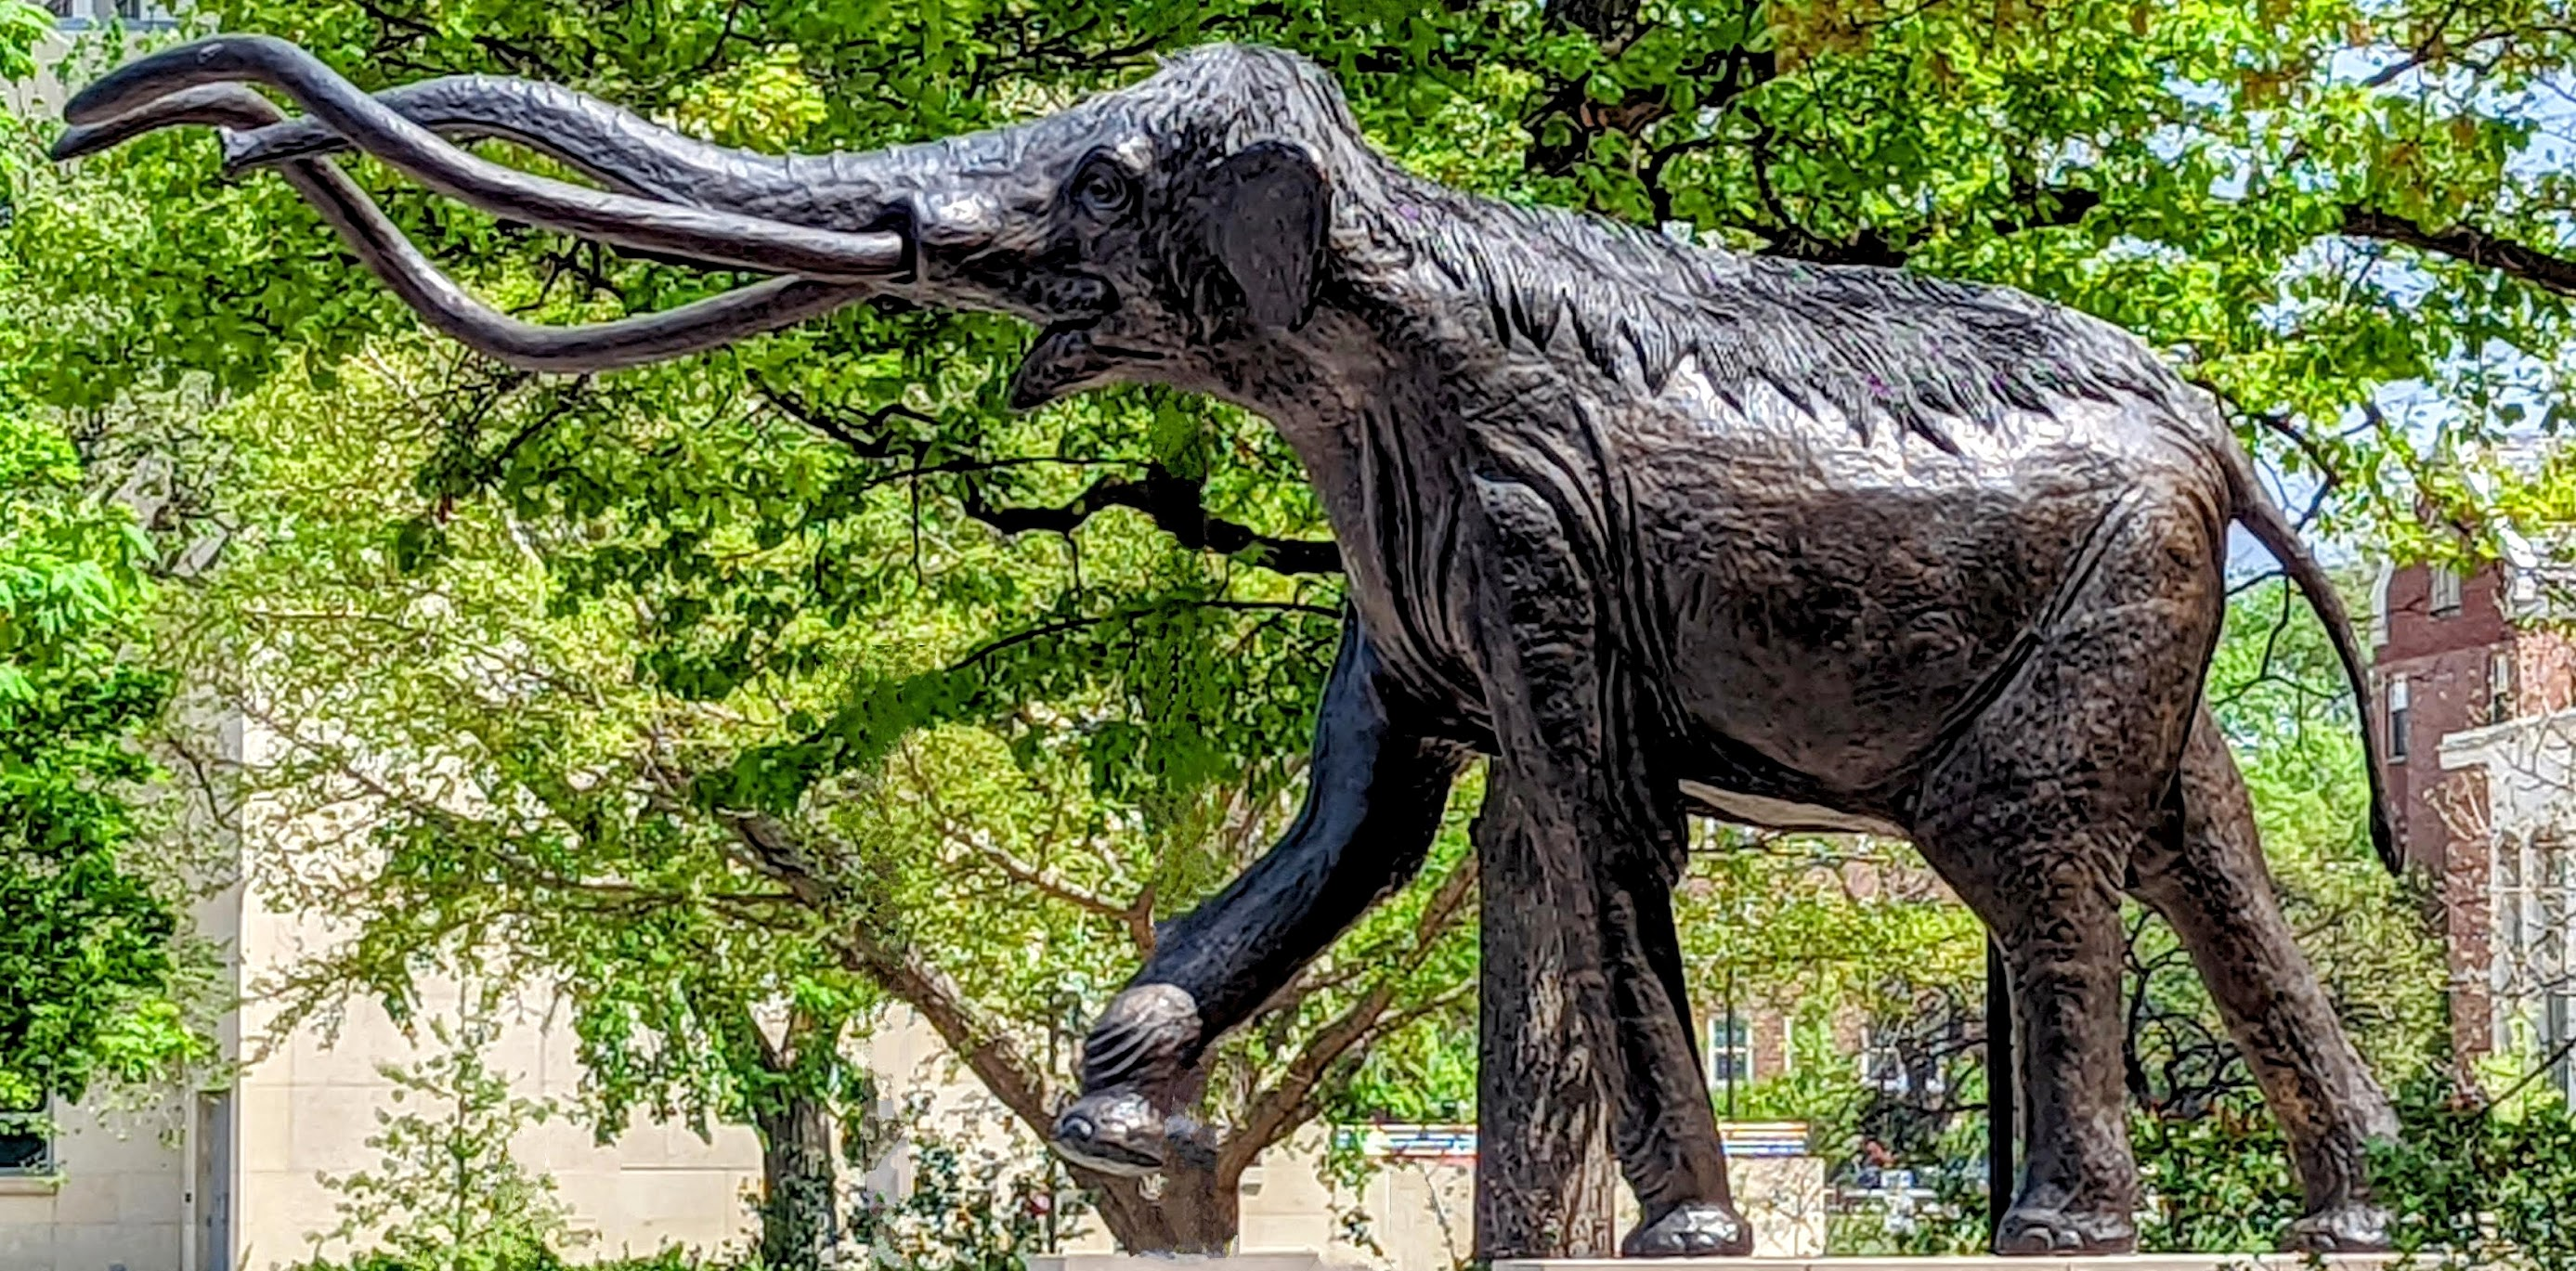
\includegraphics[width=.4\textwidth]{archie}
        \caption{Archie.\\ \footnotesize{Photograph by Bohn.}}
    \end{wrapfigure}

    You're relaxing at your favorite hangout when another customer catches your attention.
    He's rather large (dare I say, \textit{mammoth}), a bit hairy, and looking frustrated in front of his laptop.
    ``I'm Archie,'' he says, ``and I'm trying to teach myself this card game called \textit{Poker}.
    I found this source code that I thought I could use to understand Poker better, but the code is incomplete, and I don't entirely understand what's there.
    Could you explain the code to me, please?'
}

\newcommand{\GetHired}{
    Archie's face lights up in a very big smile.
    ``Thanks!''
    After pausing in thought for a moment, he says, ``Say, I've got a new startup company that could really use your help.
    Are you interested?
    It'll be exciting!''
}

\newcommand{\FirstDayOnTheJob}{
    \begin{wrapfigure}{r}{0.33\textwidth}
        \centering
        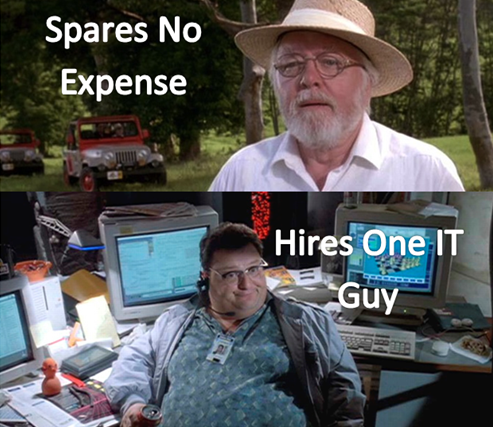
\includegraphics[width=.4\textwidth]{some-expenses-spared}
        \caption{Some expenses were spared.\\ \footnotesize{Original images \textcopyright\ Universal Studios and Amblin Entertainment, Inc. Meme creator unknown.}}
    \end{wrapfigure}

    You've recently been hired to help get the Pleistocene Petting Zoo get started.
    Your new employer, Archie, is surprisingly honest: he admits to you that some expenses were spared.
    Archie cheerfully points out that any challenge is also an opportunity to succeed.
    You suspect your job will offer plenty of ``opportunities to succeed.''
}

\newcommand{\HasKeyboard}{
    Great news!
    Archie brings you your new keyboard.
    He also brings you a problem of his own.
    Because you were held up with the broken keyboard, Archie decided to try some programming on his own, and his code is behaving strangely.
}

\newcommand{\ArchieWroteSmellyCode}{
    Working at the Pleistocene Petting Zoo certainly is proving to be interesting.
    You're glad that you don't have to worry about the problem of the giant sloths very slowly chasing their handlers, but now it seems that Archie has decided to try to write a program or two.
    At a glance, his code is smellier than the wooly rhinoceros' enclosure.
    But you take a closer look anyway to try to understand why his code acts strangely.
}

\newcommand{\InsurancePreview}{
    You hear somebody enter the room.
    ``\textit{Frankenstein}, `boat','' is the challenge, and she answers, ``borne.''
    Archie introduces you to the new arrival, ``Lil, this is our new developer, the one who wrote the app we just used.''
    He turns to you: ``This is Lilith Redd from business operations.''
    He turns back to her and continues, ``Lil, what's the good word?''

    ``The word isn't good, I'm afraid.
    I just heard back from the insurance company.''
}

\newcommand{\OnLoanToEclecticElectronics}{
    All work at the Pleistocene Petting Zoo has stopped while Archie tries to find a $\cancelto{\mathrm{reasonable}}{\mathrm{gullible}}$ insurance company.
    Rather than furloughing staff, he's asked everybody to help out with his other startup companies for a week or two.
    He specifically asked that you help out with Eclectic Electronics.

    Herb Bee, the chief engineer, explains that Eclectic Electronics is developing a patent-pending C-licon tool that will convert C code into an integrated circuit that has the same functionality as the original C code.
    To test it out, he tasked you with writing the code to implement an Arithmetic Logic Unit (ALU).
    Your task will be to implement integer addition, subtraction, multiplication, and division.
    Even though high-level languages' \textit{logical} boolean operations normally are not part of an ALU, Herb wants you to include these in the ALU to see if that can make some programs run faster.
    Because bitwise operations and bit shift operations have been implemented, you will be able to use C's bitwise and bit shift operators, but because arithmetic operations have not yet been implemented, you cannot use C's arithmetic operators.
    Because C library functions generally make use of arithmetic operations (which have not yet been implemented), you cannot use library functions.
}

\newcommand{\SuccessfulALU}{
    Herb smiles as he hands you the the test results from the latest integrated circuit fab batch.
    ``C-licon successfully turned your code into an ALU.
    Nicely done!''
    I think maybe it's time to use C-licon to see if we can improve the Floating Point Unit (FPU) on our experimental microprocessor.
}

\newcommand{\WriteAnFPU}{
    Herb tells you that, Eclectic Electronics tested the integrated circuit that the C-licon tool created from your ALU code, and they've concluded that C-licon is ready to use for their new experimental microprocessor.
    He tasks you with writing C code (that will be used by the C-licon tool) to implement a Floating Point Unit (FPU).
    Your task will be to implement floating point addition, subtraction, multiplication, and division.
    You can use any bit operations and, thanks to the ALU you wrote, you can use any integer arithmetic operations (use the conventional + - * / operators).
    Because the FPU has not yet been implemented, you cannot use C's floating point operations, you cannot use \lstinline{float}s nor \lstinline{double}s, and you cannot use library functions.
}

\newcommand{\GoingBackToTheZoo}{
    Lil enters the room.
    Herb challenges her: ``\textit{Gulliver's Travels}, `endian','' and Lil answers, ``ends.''

    Lil walks up to you and says, ``We have the insurance situation taken care of, and it's time to get the Zoo ready for guests.
    We're reassembling the tech team, and there's plenty of work to do.''

    You smile.
    ``That's good news!''

    Lil's face is hard to read.
    ``Well, yes and no.
    It's good that you'll be able to resume work on the Zoo's systems.
    But while Archie was waiting for us to fix the insurance situation, he got bored and -- cutting a long story short -- he ended up creating some new `opportunities' that we need you `to succeed' at.''
}

\newcommand{\SettledIntoRoutine}{
    You've settled into a comfortable routine at the Pleistocene Petting Zoo.
    While your job isn't quite as exciting as that of the saber-toothed tigers' dentist, it still has something new and interesting almost every day.

    Archie announces that he heard that hand-crafted assembly code can be faster than high-level language code.
    You try to explain that while this may have been true decades ago, modern optimizing compilers generate code faster than what a typical programmer can achieve with assembly code.
    Archie doesn't believe you and insists that you write the zoo's new cipher program in x86 assembly code.
}

\newcommand{\NewmanRanOffWithSamples}{
    Archie is hurriedly packing is trunk, like he's about to leave on a short-notice urgent trip.
    Before charging out the door, he pauses to tell you, ``Newman just stole some of our samples.
    I need to track him down before he sells them to the Supersized Safari Syndicate.
    I guess this means you're in charge of the Zoo's computer system now.
    Don't worry, you'll be fine. What could possibly go wrong?''
}

\newcommand{\BombLabIntroduction}{  % Ties Bryant & O'Halloran's Bomb Lab into the Pleistocene Petting Zoo story
    In a jarring collision of movie franchises, the CEO of Virtucon makes a Zoom call to the Pleistocene Petting Zoo.
    For some reason that nobody really explains, you're the only person available to handle the situation.
    The guy, who sounds kind of like an animated ogre, demands that the Pleistocene Petting Zoo deliver to him a megalodon shark with a head-mounted laser capable of emitting a beam of pure antimatter.

    You blurt out, ``Then it's not a laser,'' and then try to explain to him that megalodons are from the Miocene epoch, and expecting to find them at the Pleistocene Petting Zoo would be as ridiculous as a Cretaceous-period tyrannosaur at a Jurassic-themed park.

    ``Zip it!'' commands the guy who kind of looks like the host of a public-access show you used to watch.
    ``Since you won't meet my demand, my minions have placed a `binary bomb' under your zoo.
    Because I like really convoluted plans, we put software on your Linux server that controls the bomb.
    If you do nothing, the bomb will explode.
    If you turn off the Linux server, the bomb will explode.
    If you go slower than 50mph, the bomb will -- no, never mind that last part.

    ``The bomb software consists of a sequence of phases.
    Each phase expects you to type a particular string on \texttt{stdin}.
    If you type the correct string, then the phase is {\em defused} and the bomb proceeds to the next phase. Otherwise, the bomb {\em explodes}.
    The bomb is defused when every phase has been defused.

    ``Your mission, which you have no choice but to accept, is to defuse your bomb before the due date.
    Good luck, and welcome to the bomb squad!''
}

\newcommand{\FoodLockersAreStuck}{
    Having saved the Zoo from Dr. Evil's binary bomb, you relax back in your chair and think about taking a break.
%SPRINGBREAK
    Maybe an entire week in which you don't have solve any problems or meet any deadlines -- that'd be real nice.
%FALLBREAK
    % Maybe 4-day weekend in which you don't have solve any problems or meet any deadlines -- that'd be real nice.

    Another Zoom call comes in.
    \textit{What now!?} you wonder as you take your feet off of the desk to answer the call.
    An uncomfortable-looking animal handler says, ``We can't unlock the food lockers.
    It's the animals' feeding time, and we can't open the food lockers!
    It's feeding time, we can't get to the animals' food, and,'' his eyes dart nervously toward the animal enclosures, ``and many of them have sharp, pointy claws and others have big, stompy feet.''
}

\newcommand{\AttackLabIntroduction}{    % Ties Bryant & O'Halloran's Attack Lab into the Pleistocene Petting Zoo story
    You managed to keep the Pleistocene Petting Zoo from blowing to smithereens, but it turns out that Dr. Evil's minions weren't too careful when they put the bomb control software on the Zoo's Linux server.
    The software that controls the food locker has been heavily damaged!
    The functions that unlock the food locker doors are still present, but there's no way to activate those functions.

    You then recall what Archie told you when he hired you: some expenses were spared.
    You run the machine code through a disassembler and quickly see that it has a buffer overflow vulnerability.
    Before the situation in the dire wolf enclosure gets too dire, you sit down and get to work.

    The \function{ctarget} code runs on an older machine that allows executable code to be present on the stack, so it's vulnerable to a conventional code injection buffer overflow attack.
    \begin{itemize}
        \item Phase 1 (\function{touch1}) unlocks the food locker so the animal handlers can prepare the food.
        \item Phase 2 (\function{touch2}) opens the doors between the food locker and the carnivore enclosures;
        you will need to pass a cookie to the function to authenticate yourself.
        \item Phase 3 (\function{touch3}) closes the doors between the food locker and the carnivore enclosures.
    \end{itemize}
    The \function{rtarget} code runs on a newer machine that does not allow executable code to be present on the stack, so you'll have to conduct a return-oriented programming attack on it.
    \begin{itemize}
        \item Phase 4 (\function{touch2)} opens the doors between the food locker and the herbivore enclosures;
        you will need to pass a cookie to the function to authenticate yourself.
        \item Phase 5 (\function{touch3}) closes the doors between the food locker and the herbivore enclosures.
    \end{itemize}
}

\newcommand{\MostAnimalsAreFed}{
    Before you take on the Phase 5, pause to consider what you have accomplished so far.
    In Phases 2 and 3, you caused a program to execute machine code of your own design.
    If {\sc ctarget} had been a network server, you could have injected your own code into a distant machine.
    In Phase 4, you circumvented two of the main devices modern systems use to thwart buffer overflow attacks.
    Although you did not inject your own code, you were able inject a type of program that operates by stitching together sequences of existing code.
    Also, all animals have been fed, the carnivores are still in their enclosure, the mammoths can't fit through the herbivore door, and only the giant sloths seem interested in very slowly escaping.
}

\newcommand{\ArchieReturns}{
    Archie returns from tracking down Newman, who'd run off with some of the Pleistocene Petting Zoo's samples shortly before Dr.~Evil's Zoom call.
    ``It turns out he didn't get very far at all,'' Archie sighs.
    ``He ran into a flock of terror birds as he was leaving, and we found him in one of the emergency shelters.

    Archie smiles. ``I trust things were uneventful while I was away?''
}

\newcommand{\PickingUpNewmansProject}{
    Archie seems genuinely surprised that Newman is refusing to go back to work.
    ``You would think that he'd be grateful for being rescued from that flock of terror birds.''
    Before you can wonder out-loud whether it would be a good idea to trust someone who had just tried to sell trade secrets to a competitor, Archie gives you your new task.

    ``Because Newman isn't cooperating, I need you to finish the project he was working on.
    As you can imagine, duplicating the genetic information for our exhibits can take a long time, and Newman realized that we might be able to duplicate the data faster if we had a concurrent program which has one thread reading from the original data and another thread writing the copy.
    Unfortunately, he ran off to sell samples to the  Supersized Safari Syndicate before finishing the duplicator.
    Right now the duplicator seems to work, but it usually makes imperfect copies.
    Have you ever seen a paleolama with two noses, four eyes, and no ears!?''
}

\newcommand{\WeNeedBetterDetection}{
    Between Newman trying to sell samples to a competitor, that weird guy almost blowing up the zoo, and the animals almost escaping, Archie is getting worried.
    ``I think we need to introduce additional protective measures.
    As useful as your challenge-response app is in helping us detect intruders, I think it's now clear that we need something that will detect someone -- or some\textit{thing} -- when they're someplace they shouldn't be, even when no one else is around.
    I've asked the team at Eclectic Electronics to put something together.''
}

\newcommand{\WeNeedBetterLocks}{
    Between Newman trying to sell samples to a competitor, that weird guy almost blowing up the zoo, and the animals almost escaping, Archie is getting worried.
    ``I think we need to introduce additional protective measures.
    As useful as your challenge-response app is in helping us detect intruders, I think it's now clear that we need something that will keep someone -- or some\textit{thing} -- out of places they shouldn't be, even when no one else is around.
    I've asked the team at Eclectic Electronics to put something together.''
}

\newcommand{\IntroduceHardware}{
    Archie walks up to you, along with Herb Bee from Eclectic Electronics.
    Herb is holding a tangled mess of electronics.
    Archie explains, ``Herb here has developed a prototype of a device that he thinks will be useful for our physical security needs, as well as a few other applications around here. He calls it the \textit{Cow Pi}.''

% TODO: parameterize based on which microcontroller is actually being used
    You look at the device in Herb's hands and see the \nano\ central to the circuit.
    ``Isn't \textit{-Pi} typically used as a suffix for circuits that use a Raspberry Pi instead of an Arduino?''

    Herb replies, ``Typically, yes, but \textit{Cowduino} isn't very punny, is it?''

    Archie chimes in, ``Maybe with the right emphasis: \textit{Cow-DOO-ino}.''

    ``That's kind of subtle, don't you think? How will people know to put the emPHAsis on that sylLAble?''

    ``I think we're getting off topic here,'' you point out.
    ``How can I help?''

    ``Oh, right,'' Herb says, ``We'd like you to kick its proverbial tires.
    Let's start off with something simple, like a number builder tool.''
}

\newcommand{\JeffGoldblum}{
    Herb looks over your work.
    ``Hmm, yes. I think this is coming along nicely.
    Let's run a few more tests.''

    Archie storms into the room.
    ``We have \textit{got} to do something about security!
    How's that doodad coming along?
    Because there's now a half-man/half-fly in the labs going on-and-on about Chaos Theory and how if we just give him a MacBook and a spaceship then he'll be able to get the Lord of Thunder to travel across the 8th Dimension.
    Is that thing just about ready?''

    Herb shakes his head, ``No, not quite yet. It should be ready in about a week.''
}

\newcommand{\DisdainfulHerb}{
    Smoke wafts from Herb's soldering iron as he looks up when you approach.
    Cleaning the iron's tip, he quotes:
    ``Somebody once said, `The three most dangerous things in the world are a programmer with a soldering iron, a hardware engineer with a software patch, and'{}'' -- he glances nervously in Archie's direction -- ``{}`a user with an idea.'\footnote{
        Rick Cook, \textit{The Wizardry Consulted}, 1995.
    }$^{\mathrm{,}}$\footnote{
        The notion of being wary of programmers wielding screwdrivers or soldering irons long pre-dated this quote, as there are apocryphal tales of people who found it easier to modify the hardware to suit the software rather than the other way around.
    }''
}

\newcommand{\NumberConversionTool}{     % Since we're now allowing `sprintf()` with the LCD1602, converting between decimal and hexadecimal is trivial; it still might be okay for 7-segment displays
    Herb gets straight to the point.
    ``We promised Archie that we'd be able to start using the Cow Pi to build systems in a week.
    So far we've tested its input/output functionality, but we still need to test its timer and also whether we can take inputs without constantly polling the input devices.
    As before, we don't need to do anything too fancy;
    let's try a number base conversion tool.''
}

\newcommand{\LessDisdainfulHerb}{
    Smoke wafts from Herb's soldering iron as he looks up when you approach.
    Cleaning the iron's tip, he notes:
    ``Somebody once said that one of the most dangerous things in the world is a programmer with a soldering iron.''\footnote{
        ``The three most dangerous things in the world are a programmer with a soldering iron, a hardware engineer with a software patch, and a user with an idea.'' -- Rick Cook, \textit{The Wizardry Consulted}, 1995.
    }$^{\mathrm{,}}$\footnote{
        The notion of being wary of programmers wielding screwdrivers or soldering irons long pre-dated this quote, as there are apocryphal tales of people who found it easier to modify the hardware to suit the software rather than the other way around.
    }
}

\newcommand{\RemoteControlledCar}{

    About this time, Archie walks by, thinking about electric carts to transport visitors around the Pleistocene Petting Zoo.
    ``They probably should be remote-controlled.''
    He looks at you and Herb, and asks, ``Do you think you could make a cart a remote-controlled cart?''

    You ask the obvious question, ``Are there carts here already?''

    Archie waves his hand in the air, dismissing that detail, ``Not yet, but could you make the remote-control?''
    
    You hestatingly summarize: ``You want a cartless remote-controlled cart?''

    Archie beamingly smiles, ``Exactly!''

    Herb jumps in, ``Yes, we'll do it.''
    Herb looks at you and adds, ``It'll give us a chance to test the Cow Pi's timer and whether we can take inputs without constantly polling the input devices.''
}

\newcommand{\LauraDern}{
    You and Herb look for Archie in the Pleistocene Petting Zoo's labs to give him the good news, and you find a blond woman wearing cargo shorts, butchering a Gilbert and Sullivan song\dots \\ \\
    \textmusicalnote\ I am the very model of a modern vice admiral \textmusicalnote \\
    \textmusicalnote\ I've information about all things paleobotanical \textmusicalnote \\
    \textmusicalnote\ And I've been up to my armpits in problems scatological \textmusicalnote \\
    \textmusicalnote\ During the regency I had experience matriarchical \textmusicalnote \\
    \textmusicalnote\ I plot space travel, normal and superluminal \textmusicalnote \\
    \textmusicalnote\ (Even if I challenge the Pauli exclusion principle) \textmusicalnote \\

    ``I don't know how these people keep getting into our labs.
    \textit{Please} tell me that you have good news,'' pleads Archie.

    ``Yes, the Cow Pi is ready for whatever you need: calculators, security systems, parking meters -- you name it,'' Herb cheerfully responds.

    ``Excellent.''
    Archie turns to you.
    ``I'd like you and Newm... no, \textit{not} Newman.
    I'd like you and someone else on the staff to get started right away.
    Here's what I'd like to have built first.''
}

\newcommand{\CalculatorNeeded}{
    ``I have various teams working on different projects around here to improve security,'' Archie reminds you.
    He glances toward the Zoo's labs, where there's now a guy who looks like the actor who portrayed the fictional actor who portrayed the Norse god Odin, trying to avoid children while wistfully talking about raising rabbits in Montana.
    You briefly wonder why there are children someplace where there are also carnivorous megafauna, and then you remember that you work at a petting zoo.
    ``What I need your team to do,'' Archie continues, ``is make a four-function calculator so that we can quickly and easily determine whether we have the correct number of specimens, or if any are missing.''
}

\newcommand{\CalculatorCounting}{
    Technicians are using your calculator to compute how many specimens are still present in the lab, and establish that all specimens are accounted for after Newman's attempted theft.
    As reports come in of facilities getting secured with Cow Pi-based locks and passages being monitored with Cow Pi-based motion sensors, Archie smiles and tells you that this was a job well done.
    With all of the excitement neatly wrapped-up and arriving at a satisfactory conclusion, you look forward to a boring career in which there's absolutely no screaming and running for your life.
}

\newcommand{\CombinationLockNeeded}{
    ``I have various teams working on different projects around here to improve security,'' Archie reminds you.
    He glances toward the Zoo's labs, where there's now a guy who looks like the actor who portrayed the fictional actor who portrayed the Norse god Odin, trying to avoid children while wistfully talking about raising rabbits in Montana.
    You briefly wonder why there are children someplace where there are also carnivorous megafauna, and then you remember that you work at a petting zoo.
    ``What I need your team to do,'' Archie continues, ``is make a combination lock so that only authorized people can get into our lab facilities.''
}

\newcommand{\CombinationLockInstalled}{
    After fastening the new electronic combination lock to the lab door, Archie smiles and tells you that this was a job well done.
    With all of the excitement neatly wrapped-up and arriving at a satisfactory conclusion, you look forward to a boring career in which there's absolutely no screaming and running for your life.
}

\newcommand{\RangeFinderNeeded}{
    ``I have various teams working on different projects around here to improve security,'' Archie reminds you.
    He glances toward the Zoo's labs, where there's now a guy who looks like the actor who portrayed the fictional actor who portrayed the Norse god Odin, trying to avoid children while wistfully talking about raising rabbits in Montana.
    You briefly wonder why there are children someplace where there are also carnivorous megafauna, and then you remember that you work at a petting zoo.
    ``What I need your team to do,'' Archie continues, ``is make a range finder that will alert us when someone -- or some\textit{thing} -- gets too close to someplace they shouldn't be.''
}

\newcommand{\RangeFinderDetecting} {
    A technician installing a new range finder outside the lab door briefly sets off the alarm, but then the range finder falls quiet and faithfully reports that nothing is approaching.
    As reports come in of facilities getting secured with Cow Pi-based locks, and of accurate speciment counts accomplished with Cow Pi-based calculators, Archie smiles and tells you that this was a job well done.
    With all of the excitement neatly wrapped-up and arriving at a satisfactory conclusion, you look forward to a boring career in which there's absolutely no screaming and running for your life.
}

../../common/assignment/linked-list-nodes.tex

\captionsetup{width=.8\linewidth}
\lstset{language=c, alsolanguage=java, numbers=left, showstringspaces=false,
    moredelim = [s][\ttfamily]{/*}{*/} % I shouldn't need this parameter!
}
%%
%%
% Credit where credit is due. Skipping line numbers from
% https://tex.stackexchange.com/questions/476100/lstlisting-line-number-gaps
\makeatletter
\let\orig@lstnumber=\thelstnumber

\newcommand\lstsetnumber[1]{\gdef\thelstnumber{#1}}
\newcommand\lstresetnumber{\global\let\thelstnumber=\orig@lstnumber}
\makeatother
%%
%%

\renewcommand{\labnumber}{\pointerlabnumber}
\renewcommand{\labname}{Pointer Manipulation Lab}
\renewcommand{\shortlabname}{linkedlistlab}
\renewcommand{\collaborationrules}{\pointerlabcollaboration}
\renewcommand{\duedate}{\pointerlabdue}
\pagelayout
\begin{document}
    \labidentifier

    \pdfbookmark[1]{Frontmatter}{frontmatter}                       In this assignment, you will write code for \runtimeenvironment\ that will use new electronic devices to interact with the physical world.

The instructions are written assuming you will edit the code in the Arduino IDE and run it on \runtimeenvironment, constructed according to the pre-lab instructions.
If you wish, you may edit the code in a different environment; however, our ability to provide support for problems with other IDEs is limited.

\section*{Learning Objectives}

After successful completion of this assignment, students will be able to:
\begin{itemize}
    \item Work collaboratively on a hardware/software project
    \item Design and implement a simple embedded system
    \item Expand their programming knowledge by consulting documentation
\end{itemize}

\subsection*{Continuing Forward}

This penultimate lab assignment does not contribute to the final lab assignment.
By integrating elements of what you learned in this course, and by demonstrating that you can review documentation to learn on your own, to design a small embedded system, you will show how much progress you have made this semester.

\section*{During Lab Time}

During your lab period, coordinate with your group partner(s) to decide on your working arrangements.
Unless you're only going to work on the assignment when you're together, you may want to set up a private Git repository that is shared with your partner(s).
With your partner(s), modify your hardware kit as described in Section~\ref{sec:hardwareMods}.
Then, think through your system's design and begin implementing it.
The TAs will be available for questions.


    \softwareengineeringfrontmatter

    \section*{Scenario}                                             \ArchieWroteSmellyCode

    \section{Assignment Summary}                                    This assignment is principally about getting comfortable when explicitly working with memory.
Being able to think about a value and a reference to that value distinctly will improve your programming skills in any language.

Before you do so, in Section~\ref{sec:archiesCode} you will examine Archie's code.
Parts of Archie's programs use code that the C standard explicitly states will result in undefined behavior.
By understanding the mistakes that Archie made, we hope that you can avoid them in your own code.

In Section~\ref{sec:challengeResponse}, you will build and use a linked list.
This will require you to allocate space for the list's nodes and manipulate pointers that connect the nodes to each other.

\ifboolexpe{not bool{allowspaghetticode}}{
    There are no particular restrictions in this assignment other than those common to most lab assignments in this course.
    You can check whether you're using a \lstinline{goto} or \lstinline{continue} statement, or whether you're using \lstinline{break} or \lstinline{return} to exit a loop, by running the constraint-checking Python script:
    \texttt{python constraint-check.py linkedlistlab.json}
}{}


    \section{Stray Values in Memory} \label{sec:archiesCode}        \subsection{Pleistocene Petting Zoo Marquee} \label{subsec:uninitializedvariables}

\transitionzero

% TODO: parameterize Archie's code
\begin{lstlisting}
/***********************************************************************
 * This program will output
 **         Welcome to the
 **    Pleistocene Petting Zoo!
 **
 ** Get ready for hands-on excitement on the count of three! 1.. 2.. 3..
 ** Have fun!
 * With brief pauses during the "Get ready" line.
 ***********************************************************************/

#include <stdio.h>
#include <unistd.h>

void splash_screen(void) {
    const char *first_line = "\t     Welcome to the\n";
    const char *second_line = "\tPleistocene Petting Zoo!\n";
    printf("%s%s\n", first_line, second_line);
}

void count(void) {
    int i;
    sleep(1);
    printf("Get ready for hands-on excitement on the count of three! ");
    while (i < 3) {
        fflush(stdout);
        sleep(1);
        i++;
        printf("%d.. ", i);
    }
    printf("\nHave fun!\n");
}

int main(void) {
    splash_screen();
    count();
    return 0;
}
\end{lstlisting}

Sometimes the output was what he expected:
\begin{verbatim}
         Welcome to the
    Pleistocene Petting Zoo!

 Get ready for hands-on excitement on the count of three! 1.. 2.. 3..
 Have fun!
\end{verbatim}

But sometimes the output was missing the
``\texttt{1.. 2.. 3..}'':
\begin{verbatim}
         Welcome to the
    Pleistocene Petting Zoo!

 Get ready for hands-on excitement on the count of three!
 Have fun!
\end{verbatim}

What mistake did Archie make?
What change to \textit{one} line will fix Archie's bug?
\begin{description}
    \checkoffitem{Place your answers in \textit{answers.txt}.}
\end{description}


\subsection{Math Doesn't Work Right \dots Or Does It?} \label{subsec:danglingPointers}

\transitionone

\begin{lstlisting}
/***********************************************************************
 * This program will add two numbers and then it will multiply two other
 * numbers. Finally, it will subtract the second result from the first
 * result.
 ***********************************************************************/

#include <stdio.h>

int *add(int a, int b) {
    int addition_result = a + b;
    return &addition_result;
}

int *multiply(int p, int q) {
    int multiplication_result = p * q;
    return &multiplication_result;
}

int main(void) {
    int *sum = add(4, 5);
    printf("sum = %d\n", *sum);
    int *product = multiply(2, 3);
    printf("product = %d\n", *product);
    printf("sum - product = %d - %d = %d\n",
                        *sum, *product, *sum - *product);
    return 0;
}
\end{lstlisting}

Archie explains that when he compiles the program with the \textbf{clang} compiler and then runs it, he gets this output:

\begin{verbatim}
sum = 9
product = 6
sum - product = 6 - 6 = 0
\end{verbatim}

And when he compiles the program with the \textbf{gcc} compiler and then runs it, the program terminates with a segmentation fault.

``I see that one compiler is giving me an incorrect answer, and the other compiler is telling me that I'm using memory in an unsafe way -- but what am I doing wrong, and why does it produce an incorrect answer?''

What mistake did Archie make?
Why does \lstinline{*sum} have the value 6 on line 25?
Why does \lstinline{*sum - *product} produce the value 0?
\begin{description}
    \checkoffitem{Place your answers in \textit{answers.txt}.}
\end{description}


    \section{Challenge and Response} \label{sec:challengeResponse}  You plug in your shiny, new keyboard, tune your satellite radio to the Greatest Hits of the 1920s, and settle in to solving a more interesting problem.

To protect against corporate espionage, you are responsible for writing code for a challenge-and-response system.
Anybody can challenge anyone else in the Pleistocene Petting Zoo's non-public areas by providing the name of a book and a word contained within the book, and the person being challenged must respond with another word from that book, based on certain rules:
\begin{itemize}
    \item All of the book's words are sorted alphabetically without regard to capitalization (for example, ``hello'' occurs after ``Hear'' and before ``HELP'')
    \item The challenge word occurs \textit{occurrences} times in the book
    \item If $occurrences$ is an odd number then the response word is the word $occurrences$ places \textbf{after} the challenge word in the alphabetized list;
    if the challenge word is less than $occurrences$ places from the end of the list then ``wrap around'' to the start of the list and resume counting
    \item If $occurrences$ is an even number then the response word is the word is ${2 \times occurrences - 1}$ places \textbf{after} the challenge word in the alphabetized list;
    if the challenge word is less than ${2 \times occurrences - 1}$ places from the end of the list then ``wrap around'' to the start of the list and resume counting
\end{itemize}

Here is a simple example.
Suppose the words in the specified book are:

\begin{center}
    \begin{tabular}{cc}
        \textit{word} & \textit{occurrences} \\ \hline
        apple       & 7 \\
        banana      & 4 \\
        carrot      & 15 \\
        date        & 3 \\
        eggplant    & 2 \\
        fig         & 6 \\
        granola     & 9 \\
        horseradish & 9 \\
        ice         & 6 \\
        jelly       & 3 \\
        kale        & 1 \\
        lemon       & 2 \\
        mango       & 8 \\
        naan        & 7 \\
        orange      & 5 \\
        pineapple   & 1 \\
        quinoa      & 11 \\
        raisin      & 4 \\
        spaghetti   & 10 \\
        tomato      & 12 \\
    \end{tabular}
\end{center}
If the challenge word is ``horseradish'' then because horseradish occurs 9 times in the book, the response word is ``quinoa,'' which is 9 places in the list after ``horseradish.''
If the challenge word is ``eggplant'' then the response is ``horseradish,'' which is 3 places ($2 \times 2 - 1 = 3$) later in the list than ``eggplant.''
If the challenge word is ``quinoa'' then the response word is ``horseradish,'' because the response word should be 11 places after ``quinoa,'' but the end of the list is 3 places later;
``horseradish'' is in position 8 in the list ($11 - 3 = 8$).
(\textit{Note:} ``horseradish'' and ``quinoa'' being each other's response words is coincidental.
Unusual things happen with short lists of words that do not generalize to longer lists.)

You break the problem down into four sub-problems:

\begin{enumerate}
    \item Designing the Data Structure and Its Algorithms
    \item Alphabetizing Words
    \item Inserting Words
    \item Responding to a Challenge
\end{enumerate}

\subsection*{The Books}

Four small ``books'' are included with the starter code:

\begin{itemize}
    \item ``Animals'' (sorted, 7 words)
    \item ``Plants'' (unsorted, 7 words)
    \item ``Cars'' (sorted, 74 words)
    \item ``Food'' (unsorted, 125 words)
\end{itemize}

Two real books have also been reduced to one word per line:\footnote{The text for these books was obtained from \href{https://www.gutenberg.org/}{Project Gutenberg}.
In accordance with Paragraph~1.C of the \href{https://www.gutenberg.org/policy/license}{Project Gutenberg License}, all references to Project Gutenberg have been removed from the ``derived works'' that we are distributing.
(Removing the references to Project Gutenberg was also necessary to ensure that \textit{only} the words from the books are used for the challenge-and-response system.)}

\begin{itemize}
    \item Mary Shelly's \textit{Frankenstein; Or, The Modern Prometheus} (filename ``Frankenstein'') \url{https://www.gutenberg.org/ebooks/84} (sorted, 74,363 words)
    \item Arthur Conan Doyle's \textit{The Lost World} (filename ``TheLostWorld'')
    \url{https://www.gutenberg.org/ebooks/139} (unsorted, 77,268 words)
\end{itemize}

The very small files of 7 words can be useful for debugging, and the moderate-sized files of 74--125 words should give you confidence in the correctness of your solution.
The real books of more than 74,000 words will be useful to reveal whether you have any memory leaks in your code.
The files marked as \textit{sorted} have all of their words already in alphabetically sorted order, ignoring capitalization;
the files marked as \textit{unsorted} do not have their words sorted (the words in ``Plants'' and ``Food'' are in a randomly-selected order;
the words in ``TheLostWorld'' appear in the order that they appear in the original \textit{The Lost World}).

Each book file, ``\textit{file}'', has a corresponding ``\textit{file}-table.md'' that contains a Markdown-formatted table of the challenge words, the number of occurrences for each challenge word, and the corresponding response word.
You may use these files to confirm the correctness of your solution.

Throughout the assignment, we note that if building the list takes more than a few seconds, there is a bug in your code;
for context, we can build the list for \textit{Frankenstein} in 1--2 seconds and the list for \textit{The Lost World} in 1.5--3 seconds.
We can locate a word (or determine the absence of a word) in the \textit{Frankenstein} list in under 0.5ms and in the \textit{The Lost World} list in under 0.9ms.
Your code may take longer, but it should not take much longer.

You will earn most of the credit for this lab if your code works for pre-sorted files of up to 200 words.
The remaining credit is for making your code work with unsorted files and, when using files of up to 80,000 words, your code can generate a list and find a word in fewer than 20 seconds.

\subsection{Differences and Similarities between Java and C that are Relevant to this Assignment}

In some regards, Java keeps things simple: every variable is a reference, except when it isn't.
In other regards, C keeps things simple: you always know whether the variable you're using is a value or a pointer.

\subsubsection{Comparing Strings}

You probably learned that when comparing Java Strings, using the equality operator \lstinline{==} is error-prone.
When comparing two String literals (or variables assigned to String literals), the equality operator usually acts as a naive programmer would expect:
\lstinline{"abc" == "abc"} evaluates to \lstinline{true}.
When one or both of the Strings are generated at runtime, such as from user input, then the equality operator rarely evaluates to \lstinline{true}:
\lstinline{userInput == "abc"} will evaluate to \lstinline{false} even when the user entered ``abc''.

The reason for this is that when comparing objects (other than boxed types), Java's comparators compare the objects' references;
that is, Java comparators compare the objects' memory addresses.
Using the \lstinline{==} operator to compare Strings evaluates to \lstinline{true} only when the two Strings occupy the same address;
that is, they are both literally the same String object.
This is why you were taught to use Java's \function{String.equals()} method to compare strings.

Comparing C strings' variables has the same pitfall:
because the string variables are pointers to the first character in their respective strings, using arithmetic comparators will compare the strings' addresses.
If you want to compare two C strings, you would use the \function{strcmp()}\footnote{See footnote~\ref{note:stringFunctions}.} function.
The wrinkle is that \function{strcmp()} returns \lstinline{0} (\textit{i.e.}, \lstinline{false}) when the two strings are equal;
you will often see the idiom \lstinline{if (!strcmp(string1, string2)) {}.

The \function{strcmp(string1, string2)} function actually performs a lexicographic comparison of the strings, returning a negative value if \lstinline{string1} occurs alphabetically earlier than \lstinline{string2}, zero if every character in the two strings match, and a positive value if \lstinline{string1} occurs alphabetically later than \lstinline{string2}.
In this regard, C's \function{strcmp()} function is more like Java's \function{String.compareTo()} method than \function{String.equals()}.

\subsubsection{Copying Strings}

Because Java Strings are immutable objects, you can safely copy a string by simply copying its reference (this is called \textit{aliasing}).
You can safely write the statement \lstinline{string1 = string2;} without worrying about changes to \lstinline{string2} causing changes in \lstinline{string1}
(if you were to make changes to \lstinline{string2}, it would result in a new String object being assigned to the \lstinline{string2} variable).

For mutable objects, creating an alias (that is, copying the reference) results in the situation that changes made through one variable are visible through the other variable.
For example, if you have the statements \lstinline{list1 = list2; list2.add(foo);} then \\ \lstinline{list1.size() == list2.size() && list1.contains(foo)} will evaluate to \lstinline{true}.
If the object's class implements the \lstinline{Cloneable} interface then you can make a copy of an object without aliasing it.
If you have the statements \lstinline{list1 = list2.clone(); list2.add(foo);} then \lstinline{list1.size() == list2.size()} will evaluate to \lstinline{false}.

In general, C strings are mutable.\footnote{
    The exceptions are string literals, which are immutable, and strings declared as a pointer to a constant, which if treated as mutable will result in undefined behavior.
}
This means that you generally don't want to create an alias.\footnote{
    Sometimes you can't create an alias.
    If the left-hand-side of an assignment is a constant pointer or is effectively a constant pointer -- such as an array inside a struct -- then it cannot be re-assigned.
}
Instead, use the \function{strcpy(destination, source)} or \function{strncpy(destination, source, n)}\footnote{See footnote~\ref{note:stringFunctions}.} function to copy the \lstinline{source} string into the memory pointed to by \lstinline{destination}.
The \function{strcpy()} function will continue copying until encountering the terminating \lstinline{NUL} in the \lstinline{source} string -- this is very slightly faster (not enough that you'd notice) but is safe only if you can prove that \lstinline{destination} has enough memory allocated for the string.
The \function{strncpy()} function will copy until encountering the terminating \lstinline{NUL} or until it has copied $n-1$ characters (after which it will append a terminating \lstinline{NUL}) -- this is safer because you can ensure that the string copied to \lstinline{destination} will fit within the space allocated for it.

\subsubsection{Allocating and Deallocating Memory}

As we'll note in Section~\ref{subsubsec:equivalentJava}, Java's \lstinline{new} keyword allocates space for the new object, inferring the amount of space needed based on the class's definition.
In C, you use the \function{malloc()} function to allocate space\footnote{
    There are a small handful of alternate functions, each with their own use cases, but \function{malloc()} is most-suitable for this lab.
}, and you must be explicit about how much space you need.
An idiom is to combine \function{malloc()} with the \function{sizeof()} function, as you saw in PokerLab, and as you'll see near the start of Section~\ref{subsubsec:cImplementation}.

Java uses a \textit{garbage collector} to reclaim memory allocated for objects that are no longer in use.
The unpredictability of when garbage collection happens makes an automatic garbage collector unsuitable for many of C's uses.
For this reason (among others), the programmer is responsible for deallocating memory that is no longer needed.
This is done with the \function{free()} function.

While a variable will go out of scope at the end of the code block in which it was declared, memory allocated in that code block persists unless explicitly \function{free}d.
Once the last pointer pointing to that memory goes out of scope, you no longer have a way to \function{free} that memory, resulting in a \textit{memory leak}.
On the other hand, \function{free}ing memory while it is still being used by another pointer can result in undefined behavior.
This requires careful thought to make sure that you \function{free} all memory that you allocated, but only after it is safe to do so.

For many short-running programs, such as those you often write in school, you often can ignore the need to \function{free} allocated memory since all the program's memory will be reclaimed by the operating system when the program terminates.
A member of the C Standard Committee recently described this as having a maid that will clean up your mess.\footnote{
    \url{https://twitter.com/__phantomderp/status/1619322783162568705}, \\ \url{https://twitter.com/__phantomderp/status/1619323139665846273}
}

I advise you not to rely on that ``maid'' even for a ``short-running program,'' such as this one.
In an earlier version of this lab, there were a dozen or so students whose code, when tested against a 75,000-word file, would quickly consume all the server's physical memory.
As the first of these programs thrashed the virtual memory system, it prevented other services from working effectively, including the one that I had precautionarily introduced to kill a test after a couple of minutes.
It consumed enough resources that the system administrator couldn't log in to determine why the server had slowed to a crawl.
As I was already logged in, I was able to kill the process as the system administrator was preparing to disconnect the server from the power line.
The system administrator later commented about the resources it consumed, ``You ought never to see a `T' in the memory column'' (Figure~\ref{fig:tooMuchMemoryUsed}).

\begin{figure}
    \center
    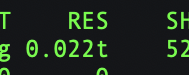
\includegraphics{too-much-memory-used}
    \caption{Screenshot showing a student's program consuming 0.022 terabytes of physical memory;
    the allocated virtual memory is not visible in the image.\label{fig:tooMuchMemoryUsed}}
\end{figure}

\subsubsection{Idioms for Defining and Initializing \texttt{Struct} Types}

In PokerLab, you worked with a struct that was defined by \lstinline{typedef} as a new type.
In this lab, you will work with a struct defined simply as a \lstinline{struct}, without a \lstinline{typedef}.
There are compelling arguments for and against both approaches in different use cases.
You should learn to be comfortable with both approaches.

In this lab, the function that initializes a node is also responsible for allocating space for that node.
In PokerLab, you saw the other idiom, in which the calling function is responsible for allocating space and passing the pointer to the initializer (this pointer is analogous to Java's implicit \lstinline{this} parameter).
The approach of having the caller allocate space seems to be more common, but both approaches are common enough to be aware of both.
(The third idiom is not to have a separate initializing function;
I discourage this approach.)

\subsection{Designing the Data Structure and Its Algorithms}

You decide that a circular linked list is the best data structure option for the challenge-and-response system.
You probably learned about linked lists in \cstwo; however, we will provide a refresher.

\subsubsection{Singly-Linked List} \label{subsubsec:singlylinkedlist}

A \textit{linked list} is a linear collection of data.
Like an array, each element (or \textit{node}) has a particular position in the list, and when you iterate over the list, you always access the elements in the same order every time (unless you change or re-order the elements).

In an array, the elements are contiguous in memory, and you can access a specific element by indexing the array (or, equivalently, performing pointer arithmetic).
In a linked list, however, the nodes can be in arbitrary locations in memory, and the nodes are connected by references (in C, pointers).
You can access a specific element only by following pointers from one node to the next until you reach the desired node.

The simplest linked list is a \textit{singly-linked list}.
A node consists of a \textit{payload} (the data that we care about) and a reference to the \textit{next} node;
see Figure~\ref{fig:singly-linked-list}.

\begin{figure}[h]
    \centering
    \begin{tikzpicture}[x=1.5mm, y=1.5mm]
        \draw[-stealth,very thick,magenta](-19,-3) -- (-10,0);
        \sllnode{0}{0}{0}
        \draw[-stealth,very thick,magenta](5,-5) -- (20,0);
        \sllnode{30}{0}{0}
        \draw[-stealth,very thick,magenta](35,-5) -- (50,0);
    \end{tikzpicture}
    \caption{Nodes in a singly-linked list consist of the payload data and a reference that points to the next node.}\label{fig:singly-linked-list}
\end{figure}

A linked list's greatest advantage over an array is that inserting and removing a node at an arbitrary location takes constant time, whereas inserting an element into an array (assuming there is sufficient memory allocated for the array) or removing an element from an array requires moving all the elements that follow the element's index.
Inserting a new node, $C$ between adjacent nodes $A$ and $B$ (where $B = A.next$) requires connecting $C.next$ to $B$ and re-assigning $A.next$ to $C$;
see Figure~\ref{fig:sll-insertion}.

\begin{figure}[h]
    \centering
    \begin{tikzpicture}[x=1.5mm, y=1.5mm]
        \draw[-stealth,very thick,magenta](-19,-3) -- (-10,0);
        \sllnode{0}{0}{0}
        \draw[-stealth,very thick,magenta](5,-5) -- (13,-5) -- (13,-12.5) -- (0,-12.5) -- (0,-25) -- (5,-25);
        \sllnode{15}{-25}{0}
        \draw[-stealth,very thick,magenta](20,-30) -- (30,-30) -- (30,-12.5) -- (17,-12.5) -- (17,0) -- (20,0);
        \sllnode{30}{0}{0}
        \draw[-stealth,very thick,magenta](35,-5) -- (50,0);
    \end{tikzpicture}
    \caption{Inserting a new node into a singly-linked list only requires assignments to the affected \textit{next} pointers.}\label{fig:sll-insertion}
\end{figure}

As with an array, you do need to maintain a variable that points to the list.
Conventionally, this is a reference to the \textit{head} of the list.
(Note that if a new node is inserted before the current head node, then the new node becomes the head of the list, and your \lstinline{head} variable would need to be updated.)
It is not uncommon to also maintain a reference to the \textit{tail} of the list.

\subsubsection{Circular Linked List} \label{subsubsec:circularlinkedlist}

A \textit{circular linked list} is a linked list in which the tail's \textit{next} field points to the head of the list.
In essence, a circular linked list has no head (because every node is some node's \textit{next}), and has no tail (because every node's \textit{next} is non-NULL);
see Figure~\ref{fig:circular-linked-list}.

\begin{figure}[h]
    \centering
    \begin{tikzpicture}[x=1.5mm, y=1.5mm]
        \sllnode{0}{30}{0}
        \draw[-stealth,very thick,magenta,rotate=0](5,25) -- (25.5,18.8);
        \sllnode{0}{30}{-72}
        \draw[-stealth,very thick,magenta,rotate=-72](5,25) -- (25.5,18.8);
        \sllnode{0}{30}{-144}
        \draw[-stealth,very thick,magenta,rotate=-144](5,25) -- (25.5,18.8);
        \sllnode{0}{30}{144}
        \draw[-stealth,very thick,magenta,rotate=144](5,25) -- (25.5,18.8);
        \sllnode{0}{30}{72}
        \draw[-stealth,very thick,magenta,rotate=72](5,25) -- (25.5,18.8);
    \end{tikzpicture}
    \caption{A circular linked list does not have a well-defined head and tail.}\label{fig:circular-linked-list}
\end{figure}

You still need to maintain a variable that points to \textit{some} node in the list.

\subsubsection{Equivalent Java Code} \label{subsubsec:equivalentJava}

In Java, you probably wouldn't implement your own linked list;
instead, you would use \lstinline{java.util.LinkedList}, which has been available since J2SE~1.2
(ignoring for the moment that Java's standard library doesn't have a circular linked list).
A list of hypothetical \lstinline{Payload} objects would be created with:
\begin{lstlisting}[numbers=none]
    List<Payload> payloads = new LinkedList<>;
\end{lstlisting}

C doesn't have a built-in linked list data type, so you will need to design one.
Let us consider what a custom linked list would look like in Java.

\begin{lstlisting}[mathescape=true]
public class Node {
    private final String word;          $\label{code:javaWord}$
    private int occurrences;            $\label{code:javaOccurrences}$
    private Node next;                  $\label{code:javaNext}$
    private Node previous;              $\label{code:javaPrevious}$

    public Node(String word) {$\lstsetnumber{\ldots}$
        ...$\lstresetnumber\setcounter{lstnumber}{11}$
    }

    public void insertAfter(Node existingNode) {$\lstsetnumber{\ldots}$
        ...$\lstresetnumber\setcounter{lstnumber}{22}$
    }
    ...$\lstresetnumber\setcounter{lstnumber}{98}$
}
\end{lstlisting}

Creating and inserting a new node would look something like this:

\begin{lstlisting}[firstnumber=200, mathescape=true]
    Node node = new Node("eggplant");   $\label{code:newNode}$
    Node otherNode = ... // code to determine where the new node goes
    node.insertAfter(otherNode);        $\label{code:javaInsertAfter}$
\end{lstlisting}

Recall that in Java, all variables except primitive types (such as \lstinline{occurrences} on line~\ref{code:javaOccurrences}) are references.
This means that the \lstinline{next} field on line~\ref{code:javaNext} is a reference to another Node, just as we described in Section~\ref{subsubsec:singlylinkedlist}.
The payload is the \lstinline{word} and how many \lstinline{occurrences} the word has, exactly what we need for the challenge-and-response system.

Recall also that in Java, the \lstinline{new} keyword allocates space for the new object, and the constructor call -- \lstinline{Node("eggplant")} -- initializes the object.

\subsubsection{C Implementation} \label{subsubsec:cImplementation}

In \textit{challenge-response.h}, you'll see a \lstinline{struct} with the same fields as our Java example:

\lstinputlisting[linerange=19-24, firstnumber=36]{../starter-code/challenge-response.h}

In \textit{challenge-response.c}, you'll also see the \function{create_node()} function:

\lstinputlisting[linerange=23-29, firstnumber=23]{../starter-code/challenge-response.c}

As you can see, it allocates space for a new node using \function{malloc()}.
The code that you will need to add to it will copy the \lstinline{word} argument into the \lstinline{word} field and set an appropriate initial value for the \lstinline{occurrences} field.
Since we don't yet know where this node will go, set the node's \lstinline{next} pointer to point to the node itself.

The other function you need to write now is \function{insert_after()}:

\lstinputlisting[linerange=31-36, firstnumber=31]{../starter-code/challenge-response.c}

As the name and documentation indicate, you need to add code that will update the nodes' \lstinline{next} pointers so that \lstinline{new_node} is placed in the list immediately after \lstinline{existing_node}.
You can ignore the \lstinline{previous} pointers for this assignment.

Two notes:
\begin{itemize}
    \item The header comment notes that ``If \lstinline{existing_node}'s original \lstinline{next} is non-NULL, then that will become \lstinline{new_node}'s \lstinline{next}.''
            In the case of the circular linked list used in this lab, \lstinline{existing_node}'s \lstinline{next} pointer \textit{must} be non-NULL, and so you do not need to check for NULL \lstinline{next} pointers.
    \item There is another function, \function{insert_before()}, which you do not need to implement in this lab.
\end{itemize}

After you have implemented \function{create_node()} and \function{insert_after()}, go to the \function{main()} function in \textit{linkedlistlab.c} and un-comment the call to \function{test_linked_list_functions()}.

\lstinputlisting[linerange=58-59, firstnumber=58]{../starter-code/linkedlistlab.c}

Build the executable with the command: \texttt{make}.
Be sure to fix both errors and warnings.
When the program compiles without generating any warnings or errors, run it with the command \texttt{./linkedlistlab}.
The output should indicate a list with the nodes in the order of ``first node,'' ``fourth node,'' ``second node,'' and ``third node.''

\subsection{Change All Uppercase Letters to Lowercase}

%In Problem~2, you wrote code to convert uppercase letters to lowercase letters.
Add code to \function{word_to_lowercase()} that calls that function to convert all letters in a word to lowercase letters.
%\textbf{(Do not copy the \function{to_lowercase()} function into \textit{challenge-response.c};
%we will link to the function in \textit{problem2.c})}.
Unlike KeyboardLab, you may use C's \function{tolower()} function\footnote{See \S7.8.2 and \S{}B.2 of Kernighan \& Ritchie's \textit{The C Programming Language}, 2nd ed.} to convert uppercase letters to lowercase letters.

\lstinputlisting[linerange=48-62, firstnumber=48]{../starter-code/challenge-response.c}

The starter code includes a function to compare two words (you do not need to write this function) but it assumes that both words are completely lowercase.

%If you have not completed Problem~2, then place this code in your \textit{problem2.c} file so that you can work on Problem~5
%(note that this code violates Problem~2's constraints):
%
%\begin{lstlisting}
%#include <ctype.h>
%
%char decapitalize(char character) {
%    return tolower(character);
%}
%\end{lstlisting}

\subsection{Inserting Words} \label{subsec:inserting-words}

Comment-out (or delete) the call to \function{test_linked_list_functions()}.

For this sub-problem, the user will be prompted to enter the name of a book, which will be the filename of a file that contains all of the book's words.
All punctuation has already been removed from the files, and each line in the file contains exactly one word.
For this assignment, you only need to work with files whose contents are already sorted.

\lstinputlisting[linerange=67-90, firstnumber=67]{../starter-code/challenge-response.c}

Add code to \function{insert_word()}\footnote{\function{insert_word()}'s header comment says that the head of the list is the node with alphabetically-earliest word.
    For a circular linked list, you can write a perfectly-functional implementation with the head at anyplace in the list, but our grading software assumes that the head is the alphabetically-earliest word.
    If you write code that meets the specification but is not scored correctly, see the syllabus for grade challenges.}
and \function{build_list()} to read the specified file one line at a time.\footnote{See \S7.5 and \S{}B1.1.1 of Kernighan \& Ritchie's \textit{The C Programming Language}, 2nd ed. for \function{fopen()} and \function{fclose()}, and \S7.7 and \S{}B1.1.4 for \function{fgets()}.}
For each word, convert it to lowercase, and then traverse the list to find the appropriate place for the word.
(Note that there will not be a list to traverse when your code reads the first word!)
If the word is not in the list then create a node for that word and insert it into the list at the correct location.
If there is already a node containing that word, then increment that node's variable that tracks the number of occurrences.
Be sure that \textit{only} the word is placed in a node;
specifically, do not include a newline character nor any other characters that are not part of the word.

Note that when you are working with files whose contents are already sorted, you are guaranteed that every word read from the file (other than the first word) is either another instance of the previous word that was read, or it will appear in the list immediately after the previous word that was read.
%You might use this characteristic to simplify the code to build your list if you are not attempting any extra credit.
You might use this characteristic to simplify the code to build your list for now.
Later, in Section~\ref{subsubsec:insertionsort}, you will modify your code to work with unsorted files.
For now, however, you can earn most of the assignment's points by working with the simplifying assumption of having pre-sorted files.

Build the program and correct all warnings and errors.\ When the program compiles without generating any warnings or errors, run it.
If your program requires more than a few seconds to build the list, there is a bug in your code.
If your program does not produce the expected output, the \function{print_list()} utility function will help you see the list that your code created.

\subsection{Respond to a Challenge}

You now have implemented enough of the other sub-problems that you can write the code to respond to a challenge.

\lstinputlisting[linerange=95-113, firstnumber=95]{../starter-code/challenge-response.c}

After the word list is complete (after you have inserted all words in the file), the user will be prompted to enter the challenge word.
Add code to \function{respond()} that traverses the word list to find that word.
If the word is not present in the list, return ``(word) is not present!'', where ``(word)'' is the challenge word.

%In Problem~3, you wrote code to determine whether an integer value is even.
Use the number of occurrences recorded in that the challenge word's node to find the response word as described in the challenge-and-response rules, and return that word.
%\textbf{(Do not copy the \function{is_even()} function into \textit{challenge-response.c};
%we will link to the function in \textit{problem3.c}.)}
%
%If you have not completed Problem~3, then place this code in your \textit{problem3.c} file
%(note that this code violates Problem~3's constraints):
%
%\begin{lstlisting}
%int is_even(int value) {
%    return !(value % 2);
%}
%\end{lstlisting}

If your program does not provide the response word nearly instantaneously, there is a bug in your code.

\subsection{The Final Touches}

You have now completed enough of the assignment to receive at least 19 out of 25 points.
The remaining steps will re-visit your earlier work to make improvements.
Because you will be modifying your working code, this would be a good time to make a backup copy of your code or to commit it to a private Git repository.

\subsubsection{Designing the Data Structure and Its Algorithms, Revisited: Doubly-Linked List} \label{subsubsec:doublylinkedlist}

You may be able to produce small performance improvements if you can traverse the list forward and backward by creating a circular doubly-linked list instead of a circular singly-linked list.

A \textit{doubly-linked list} is a linked list with the property that each node maintains a link not only to the \lstinline{next} node but also a link to the \lstinline{previous} node.
In C, these links are pointers.

\begin{figure}[h]
    \centering
    \begin{tikzpicture}[x=1.5mm, y=1.5mm]
        \draw[-stealth,very thick,magenta](-20,-4.25) -- (-10,0);
        \draw[stealth-,very thick,yellow](-20,0) -- (-8,-5);
        \dllnode{0}{0}{0}
        \draw[-stealth,very thick,magenta](8,-5) -- (20,0);
        \draw[stealth-,very thick,yellow](10,0) -- (22,-5);
        \dllnode{30}{0}{0}
        \draw[-stealth,very thick,magenta](38,-5) -- (50,0);
        \draw[stealth-,very thick,yellow](40,0) -- (50,-4.25);
    \end{tikzpicture}
    \caption{Nodes in a doubly-linked list consist of the payload data and references that point to the previous and next nodes.}\label{fig:doubly-linked-list}
\end{figure}

Inserting new node, $C$ between adjacent nodes $A$ and $B$ (where $B = A.next$ and $A = B.previous$) requires connecting $C.previous$ to $A$ and $C.next$ to $B$, and re-assigning $A.next$ to $C$ and $B.previous$ to $C$.

Modify your \function{insert_after()} function to update not only the \lstinline{next} pointers but also the \lstinline{previous} pointers so that \lstinline{new_node} is placed between \lstinline{existing_node} and the node that originally was located immediately after \lstinline{existing_node}.
Modify your \function{insert_after()} and \function{respond()} functions to take advantage of the \lstinline{previous} pointers.

After the program compiles without warnings or errors, you may want to use \function{print_list} to confirm that the \lstinline{previous} pointers are updated correctly.
If your program requires more than a few seconds to build the list, there is a bug in your code.

Creating a circular doubly-linked list is worth another point.
This would be a good time to make a backup copy of your code or to commit it to a private Git repository.

\subsubsection{Inserting Words, Revisited: Working with Unsorted Files} \label{subsubsec:insertionsort}

In Section~\ref{subsec:inserting-words}, you had the option of simplifying your code by treating the last word added as the head of the list instead of traversing the list to find the correct location for a word.
To work with unsorted files, you will need a way to build and maintain a sorted list -- the insertion sort algorithm is a good choice.
You might also want to modify your code to create a circular doubly-linked list.

\paragraph{Insertion Sort}

While you probably learned about sorting in \cstwo, you may not have learned about \textit{Insertion Sort}.
If you did learn about Insertion Sort, you probably learned that it's a $\mathcal{O}(n^2)$ algorithm that is less efficient than $\mathcal{O}(n \log n)$ sorting algorithms such as Merge Sort and Quick Sort.
Insertion Sort has a particular advantage in that it can be applied \textit{as the list is built}, making for a much simpler and less error-prone implementation than a different sort that requires the list to already be built.

The Insertion Sort algorithm reads an input and then traverses a sorted list to find the proper location in the sorted list for the input.
The input is then inserted into the list at that location.

Your current implementation of \function{insert_word()} might be based off of the assumption that the word is either another instance of the last word to be added to the list or is not present in the list.
Update \function{insert_word()} so that it looks for the word in the sorted list.
If the word is found in its proper location in the sorted list, then update the number of occurrences as before.
If the word is not present in its proper location in the sorted list, then insert a new node for that word at its proper location in the sorted list.
If your program requires more than a few seconds to build the list, there is a bug in your code.

Building a list of up to 200 words and generating the correct response when the ``book'' file is unsorted is worth two points (regardless of whether the list is singly- or doubly-linked).
This would be a good time to make a backup copy of your code or to commit it to a private Git repository.

\subsubsection{Inserting Words Revisited: Working with Large Files}

Your code might already be able to handle large files in just a few seconds, in which case you are finished.

On the other hand, your code might run briskly when working with smaller files of only a couple of hundred words but then become very sluggish when the number of words is in the thousands.
This tends to be due to one (or both) of two causes.
Look for inefficient algorithms, and look for memory leaks.
If you use the \texttt{top} utility while running your program, and you notice that your program is allocating more than 10MB, then you probably have a memory leak.
If your program is allocating more than 1GB, then your program most certainly has a memory leak.

Being able to generate a list from a file of up to 80,000 pre-sorted words and generating the correct response, all within 20 seconds, is worth two points.
Being able to do so from a file of up to 80,000 unsorted words is worth another point.


    \section{Turn-in and Grading}                                   \filesubmission.

\policyforcodethatdoesnotcompile

\latepolicy

\subsection*{Rubric}

This assignment is worth 35 points.
\begin{description}
    \rubricitem{1}{\function{is_nan()} correctly reports whether or not its argument is a number}
    \rubricitem{1}{\function{is_zero()} correctly reports whether or not its argument is zero}
    \rubricitem{1}{\function{is_infinity()} correctly reports whether or not its argument is infinite}
    \rubricitem{1}{\function{is_negative()} correctly reports whether or not its argument is negative}
    \rubricitem{1}{\function{get_754_integer()} correctly extracts the significand's implicit integer}
    \rubricitem{1}{\function{get_754_fraction()} correctly extracts the significand's fraction bits}
    \rubricitem{1}{\function{get_754_exponent()} correctly extracts the exponent}
    \rubricitem{1}{\function{decode()} correctly converts an \lstinline{ieee754_t} value into a \lstinline{unnormal_t} structure}
    \rubricitem{1}{\function{negate()} correctly changes its argument's sign}
    \rubricitem{5}{\function{add()} can add integers \& fractions, positive \& negative values, and ``large'' \& ``small'' numbers}
    \rubricitem{1}{The identity and commutative properties hold for \function{add()}}
    \rubricitem{1}{\function{add()} provides correct answers for its special cases}
    \rubricitem{5}{\function{multiply()} can multiply integers \& fractions, positive \& negative values, and ``large'' \& ``small'' numbers}
    \rubricitem{2}{The identity, zero, and commutative properties hold for \function{multiply()}}
    \rubricitem{1}{\function{multiply()} provides correct answers for its special cases}
    \rubricitem{1}{\function{divide()} provides correct answers for its special cases}
    \rubricitem{1}{\function{divide()} can divide when the divisor is of the form $\pm 2^n, -126 \le n \le 127$}
    \rubricitem{1}{\function{divide()} can divide when the dividend's significand is a multiple of the divisor's significand}
    \rubricitem{1}{\function{add()} demonstrates that \function{encode()} rounds down when the truncated part of the significand is less than halfway between representable values}
    \rubricitem{1}{\function{add()} demonstrates that \function{encode()} rounds up when the truncated part of the significand is more than halfway between representable values}
    \rubricitem{2}{\function{add()} demonstrates that \function{encode()} rounds to the nearest-even when the truncated part of the significand is exactly halfway between representable values}
    \rubricitem{1}{Rounding can carry into the exponent}
    \rubricitem{1}{\function{add()} and/or \function{multiply()} demonstrate that \function{encode()} overflows to infinity}
    \rubricitem{1}{\function{add()}, \function{multiply()}, and/or \function{divide()} demonstrate that \function{encode()} gracefully underflows through subnormal numbers}
    \rubricitem{1}{\function{multiply()} and/or \function{divide()} demonstrate that \function{encode() underflows to zero}}
    \bonusitem{2}{\function{divide()} can divide arbitrary values}
\end{description}

\textbf{Penalties}
\begin{description}
    \softwareengineeringpenalties
    \item[no credit] for functions that use \lstinline{float} or \lstinline{double} variables or constants, use \lstinline{union} variables, use C's floating point operations, and/or a function you did not write
    \item[no credit] for arithmetic functions, if \function{decode()} and/or \function{encode()}  use \lstinline{float} or \lstinline{double} variables or constants, use \lstinline{union} variables, use C's floating point operations, and/or a function you did not write
\end{description}


    \section*{Epilogue} \InsurancePreview

    \textit{To be continued...}

\end{document}
